\documentclass[12pt,a4paper,table]{article}

\usepackage{lmodern}
\usepackage[T1]{polski}
\usepackage[utf8]{inputenc}

\usepackage[a4paper,
            tmargin=2cm,
            bmargin=2cm,
            lmargin=2cm,
            rmargin=2cm,
            bindingoffset=0cm]{geometry}

\usepackage[table, w11colors]{xcolor}
\usepackage{tocloft}
\usepackage{hyperref}

\usepackage{amsmath}
\usepackage{amssymb}
\usepackage{siunitx}

\usepackage{listings}

\usepackage{graphicx}
\usepackage{subfig}
\usepackage{float}
\usepackage{booktabs}

\usepackage{tikz-timing}



\hypersetup{
    colorlinks,
    citecolor=black,
    filecolor=black,
    linkcolor=black,
    urlcolor=black
}

\title{Technika cyfrowa - Sprawozdanie nr 2}
\author{Bartomiej Słupik \and Przemysław Węglik \and Błażej Nowicki \and Jan Chyczyński}

\newtheorem{definition}{Def}

\begin{document}
    \maketitle    
    \section{Zadanie 2a}
    Zadanie polega na zaprojektowaniu i zbudowaniu asynchronicznego przerzutnika RS przy pomocy dwóch bramek NAND.

    \subsection{Idea}
    Układ docelowy powinien posiadać wyjścia $Q$ i $\overline{Q}$, oraz wejścia $S$ i $R$ oraz działać zgodnie z tabelą prawdy
    przedstawioną poniżej.

    \begin{figure}[h]
        \centering
        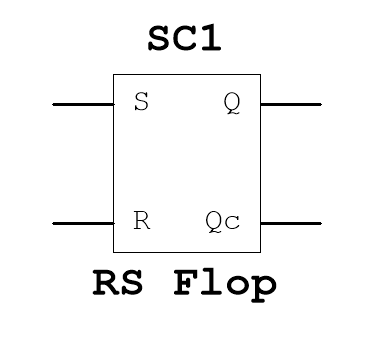
\includegraphics[width=0.3\linewidth]{images/rs_idea.PNG}
        \caption{Schemat ideowy przerzutnika RS}
        \label{fig:rs_idea}
    \end{figure}

    \begin{table}[h]
        \centering
        \begin{tabular}{|ccc|c|}
            \hline
            $S$ & $R$ & $Q$ & $Q_+$ \\
            \hline
            0   & 0   & 0   & 0     \\
            0   & 0   & 1   & 1     \\
            \hline
            0   & 1   & 0   & 0     \\
            0   & 1   & 1   & 0     \\
            \hline
            1   & 0   & 0   & 1     \\
            1   & 0   & 0   & 1    \\
            \hline
        \end{tabular}
        \caption{Tabela prawdy przerzutnika RS}
        \label{tab:rs_truthtable}
    \end{table}

    Zauważmy, że w tabeli nie pojawia się stan $S = R = 1$. Jest to tzw. stan zakazany, zatem zakładamy, że nie zachodzi.

    \subsection{Rozwiązanie teoretyczne}

    Szukamy funkcji logicznej określającej stan kolejnej iteracji $Q_+$ w zależności od stanu poprzedniego:
    \begin{equation}
        Q_+ = Q_+(S, R, Q)
    \end{equation}

    W celu znalezienia tej funkcji posłużono się tabelą Karnough:

    \begin{figure}[h]
        \centering
        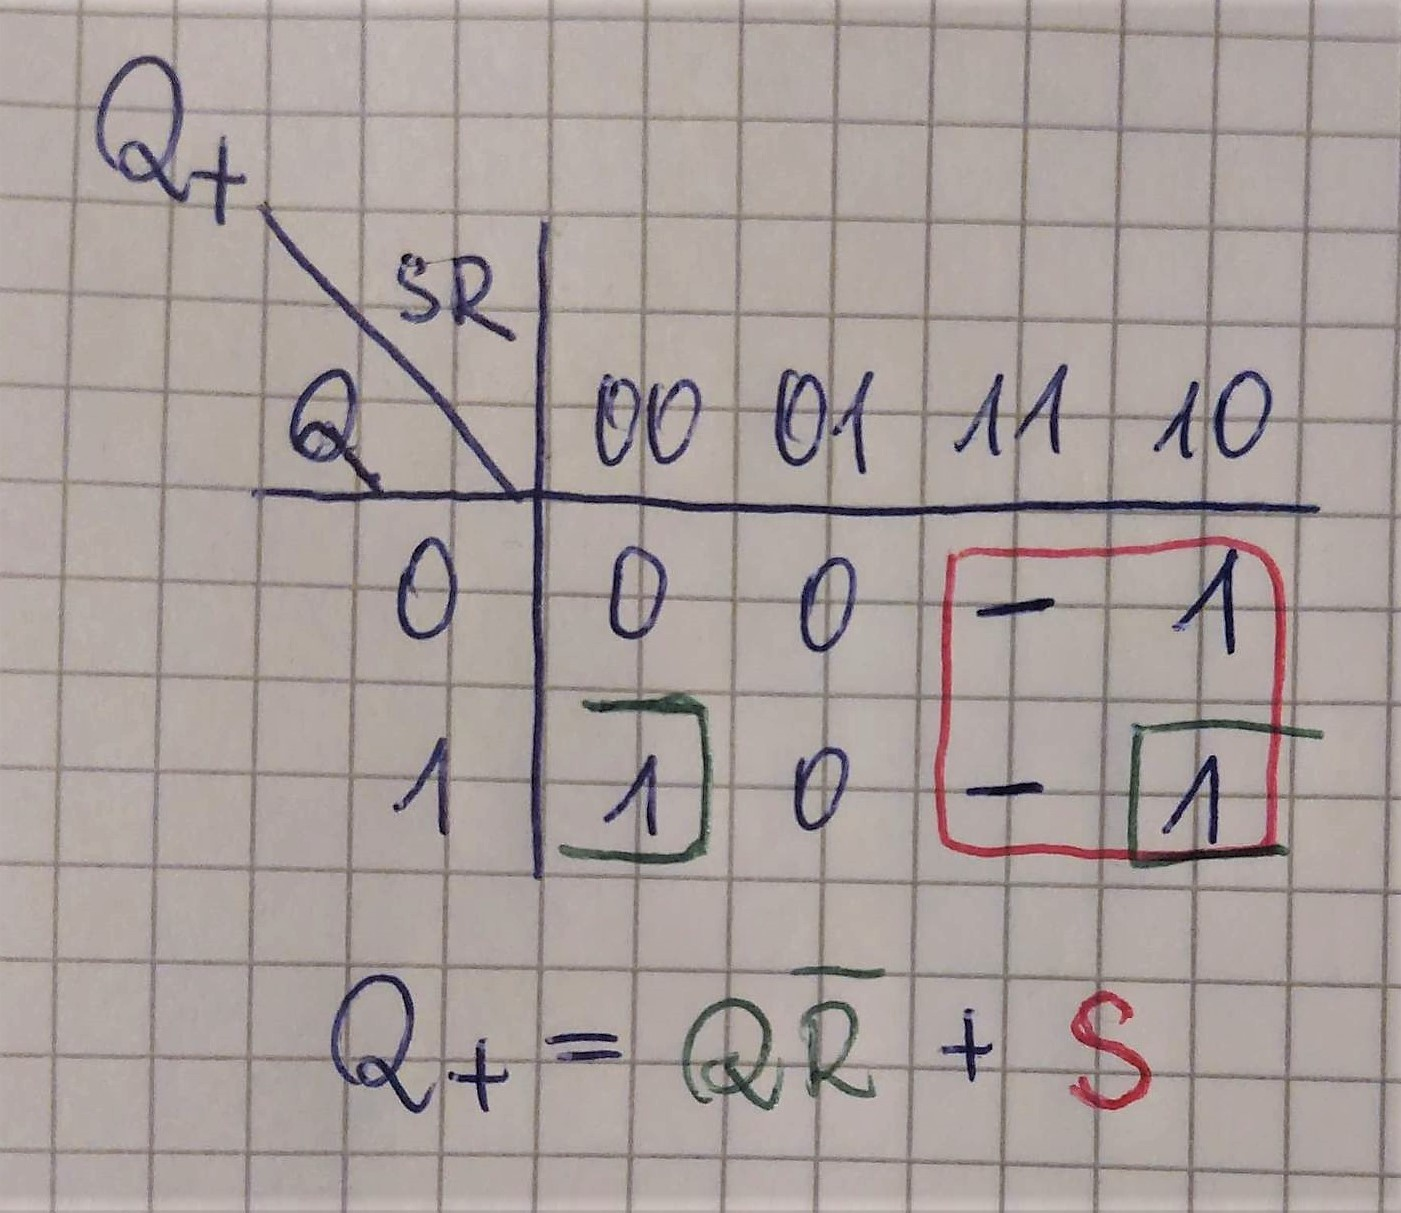
\includegraphics[width=0.3\linewidth]{images/rs_karnough.jpg}
        \caption{Tabela Karnough zastosowana w celu znalezienia funkcji logicznej przerzutnika RS}
        \label{fig:rs_karnough}
    \end{figure}

    Następnie przekształcono funkcję $Q_+$, aby zapisać ją przy pomocy funkcji NAND:

    \begin{figure}[h]
        \centering
        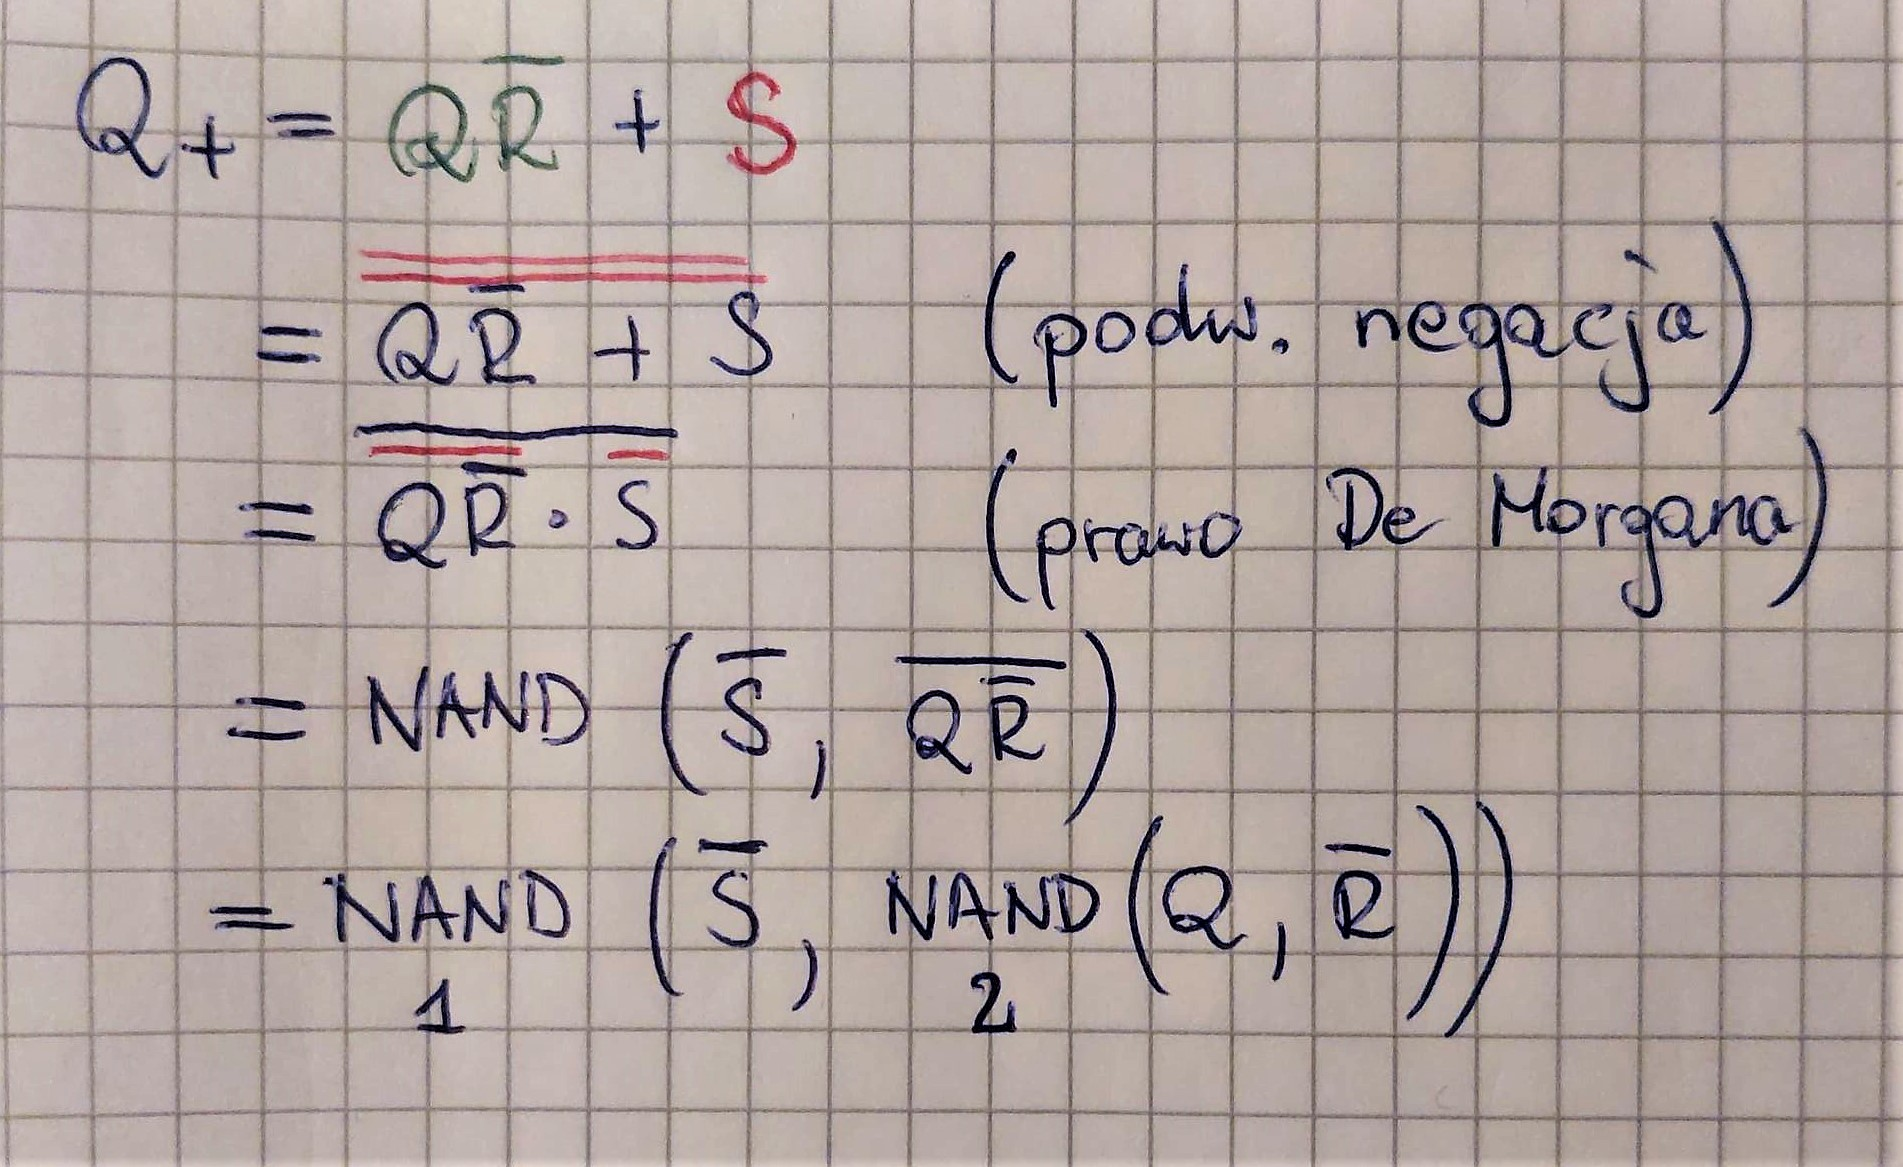
\includegraphics[width=0.6\linewidth]{images/rs_derivation.jpg}
        \caption{Przekształcenia wzoru funkcji logicznj do postaci złożonej z funkcji NAND}
        \label{fig:rs_derivation}
    \end{figure}

    Na podstawie wzoru funkcji sporządzono schemat układu, który został przedstawiony na poniższym rysunku:

    \begin{figure}[h!]
        \centering
        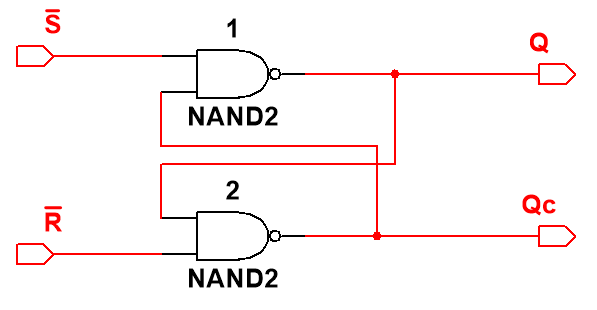
\includegraphics[width=0.5\linewidth]{images/rs_schematic.PNG}
        \caption{Schemat przerzutnika RS. Wejścia $\overline{S}$ i $\overline{R}$ są aktywne w stanie niskim.}
        \label{fig:rs_schematic}
    \end{figure}

    \subsection{Testy w programie Multisim}

    Aby przetestować zaprojektowany układ, zbudowano następujący układ testowy w programie Multisim, 
    który porównuje działanie układu z rzeczywistym przerzutnikiem RS:

    \begin{figure}[h]
        \centering
        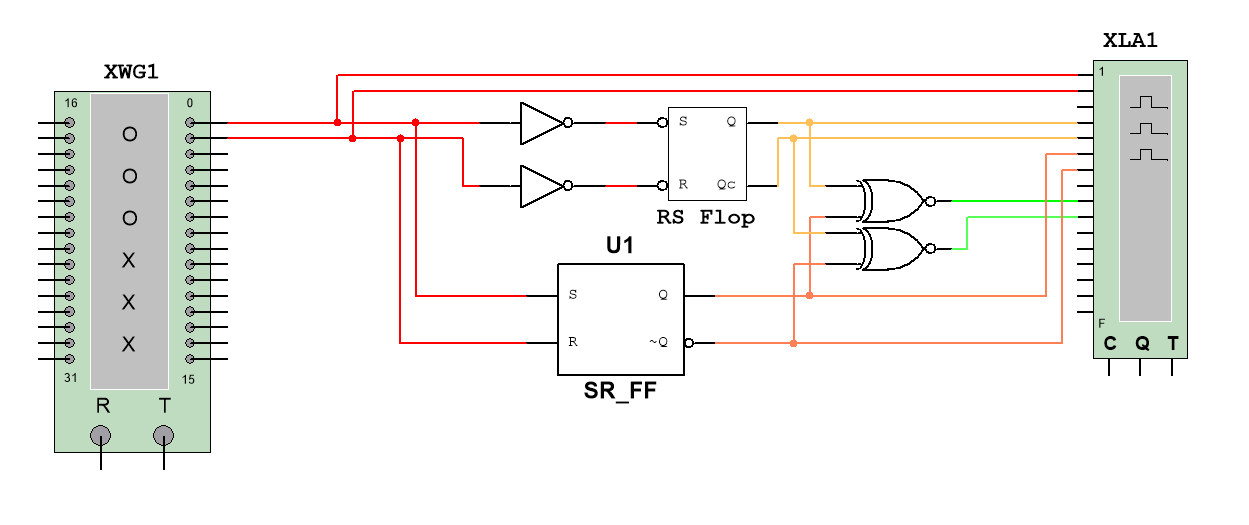
\includegraphics[width=0.9\linewidth]{images/rs_test.PNG}
        \caption{Schemat układu testowego.}
        \label{fig:rs_test}
    \end{figure}

    Generator słów bitowych ustawiono na następującą sekwencję, która testuje przejścia między wszystkimi
    możliwymi stanami:

    \begin{figure}[h]
        \centering
        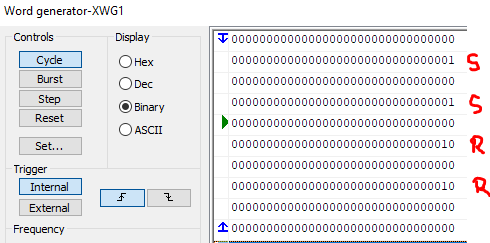
\includegraphics[width=0.6\linewidth]{images/rs_xwg.PNG}
        \caption{Sekwencja słów bitowych na wejściu układu testowego.}
        \label{fig:rs_xwg}
    \end{figure}

    Na analizatorze stanów logicznych zaobserwowano następujące dane:

    \begin{figure}[h]
        \centering
        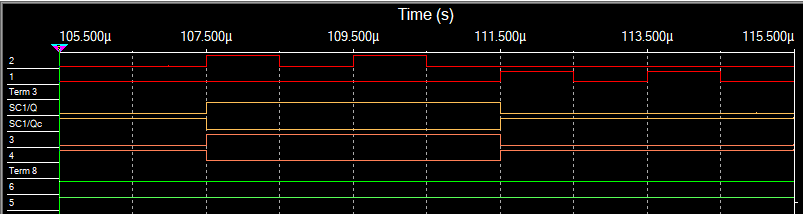
\includegraphics[width=0.8\linewidth]{images/rs_plot.PNG}
        \caption{Sekwencja słów bitowych na wejściu układu testowego.}
        \label{fig:rs_plot}
    \end{figure}

    Ciągły stan wysoki na wyjściach bramek XNOR sprawdzających równoważność układów dowodzi poprawności działania
    przerzutnika.

    \subsection{Wnioski}

    \begin{enumerate}
        \item Przerzutnik RS jest prostym ukłądem, który sprawdza się,
            gdy mamy pewność, że układ sterujący nim nie poda na wejściu stanu zabronionego $S = R = 1$. Jeśli przerzutnikiem
            steruje wprost użytkownik, lepiej zastosować przerzutnik JK, który jest odporny na niekontrolowane zachowanie.

        \item Przerzutnik RS można zastosować do budowy rejestrów przesuwnych.
        
        \item Przerzutnik RS można zastosować w celu uniknięcia "efektu skakania" przycisków i przełączników mechanicznych.
    
        \item Przerzutnik RS znajduje zastosowanie w układach czasowych, m. in. timerze NE555
    \end{enumerate}




\end{document}